\documentclass{article}
\usepackage{graphicx}
\graphicspath{{plots/}}
\usepackage{float}
\usepackage[margin=1in]{geometry}
\usepackage{hyperref} 

\title{CS422: Assignment 1 Report}
\author{Group: Kushagr Khanna, Joseph Getachew, Isaac Hallman, Marko Kovacevic}
\date{September 2026}

\begin{document}

\maketitle
\pagebreak


\section*{Repository}

\textbf{Github:} \url{https://github.com/krash3125/cs422-assignment-1}
\\\\
Plots are generated in the \texttt{matplotlib-gen.py} file

\section* {Part 1}

\subsection*{(b)}

\begin{figure}[H]
    \centering
    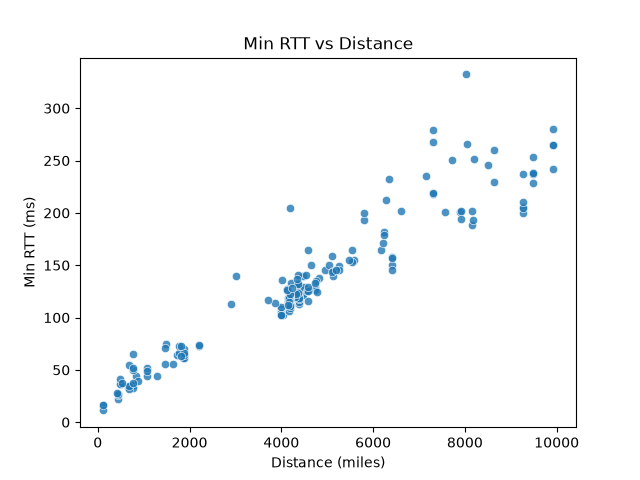
\includegraphics[width=0.8\textwidth]{min_rtt_vs_distance.png}
    \caption{Min RTT vs Distance}
\end{figure}

\begin{figure}[H]
    \centering
    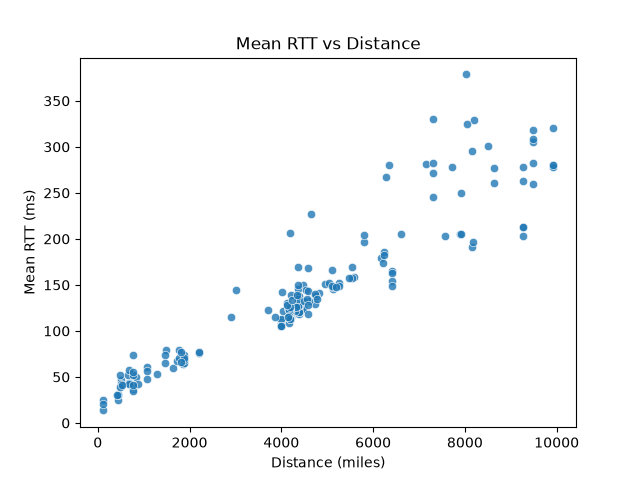
\includegraphics[width=0.8\textwidth]{mean_rtt_vs_distance.png}
    \caption{Mean RTT vs Distance}
\end{figure}

\begin{figure}[H]
    \centering
    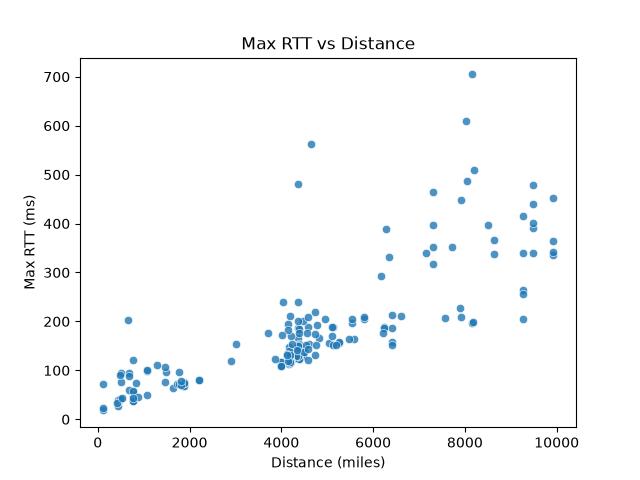
\includegraphics[width=0.8\textwidth]{max_rtt_vs_distance.png}
    \caption{Max RTT vs Distance}
\end{figure}

\subsection*{(c)}

These results make sense because the further you are from the server the more time it takes to receive a packet. It will take more time for the data to travel across the network. Min rtt is heavily correlated with distance and tells us the minimum latency to that server which can help us estimate how far away the server is. Lower min latency likely means a closer server. A high max rtt can tell us one of two things, either the server is pretty far away or the server is congested (can be a combination of both too).

\section* {Part 2}

\subsection*{(b)}

\begin{figure}[H]
  \centering
  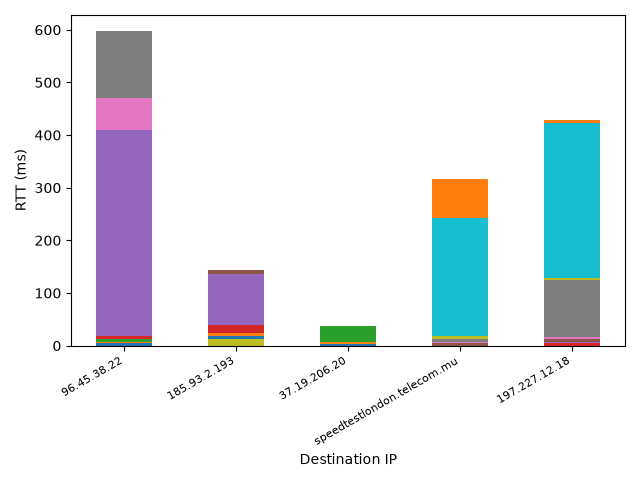
\includegraphics[width=0.8\textwidth]{stacked_bar_hops_rtt.png}
  \caption{Max RTT vs Distance}
\end{figure}

\subsection*{(c)}

\begin{figure}[H]
  \centering
  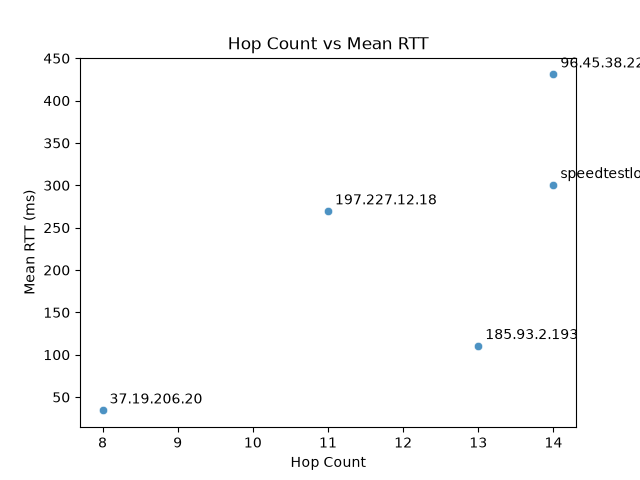
\includegraphics[width=0.8\textwidth]{hop_count_vs_rtt.png}
  \caption{Hop Count vs RTT}
\end{figure}

\subsection*{(d)}
Generally the higher the hop count the larger the rtt will be, this makes sense because the further away a server is the more hops are required to get a response back and we know already the further the server is it is more likely the rtt will be higher too.

\end{document}
